\begin{boldmath}
\chapter{Limits on $q^*$ production at a VLHC}
\label{chap:VLHC_Qstar}
\end{boldmath}

\input QstarVLHC/authorlist.tex

We look for a dijet resonance corresponding to an excited quark $q^*$
in a simulated sample corresponding to 3\,ab$^-1$ of $pp$ collisions
at $\sqrt{s} = 100$\,TeV.  Using a cut and count analysis approach we
are able to exclude $q^*$ masses upto 48\,TeV at 95\% CL,
corresponding to a length scale of around 4\,am.

\section{Introduction}

At the new energy regime afforded by a $\sqrt{s} =100$\,TeV $pp$
collider (VLHC), we search for possible structure to the quarks of the
standard model \cite{Baur:1989kv}.

\section{Data and detector simulation}

\section{Analysis}

\section{Results}

\begin{figure}
\begin{center}
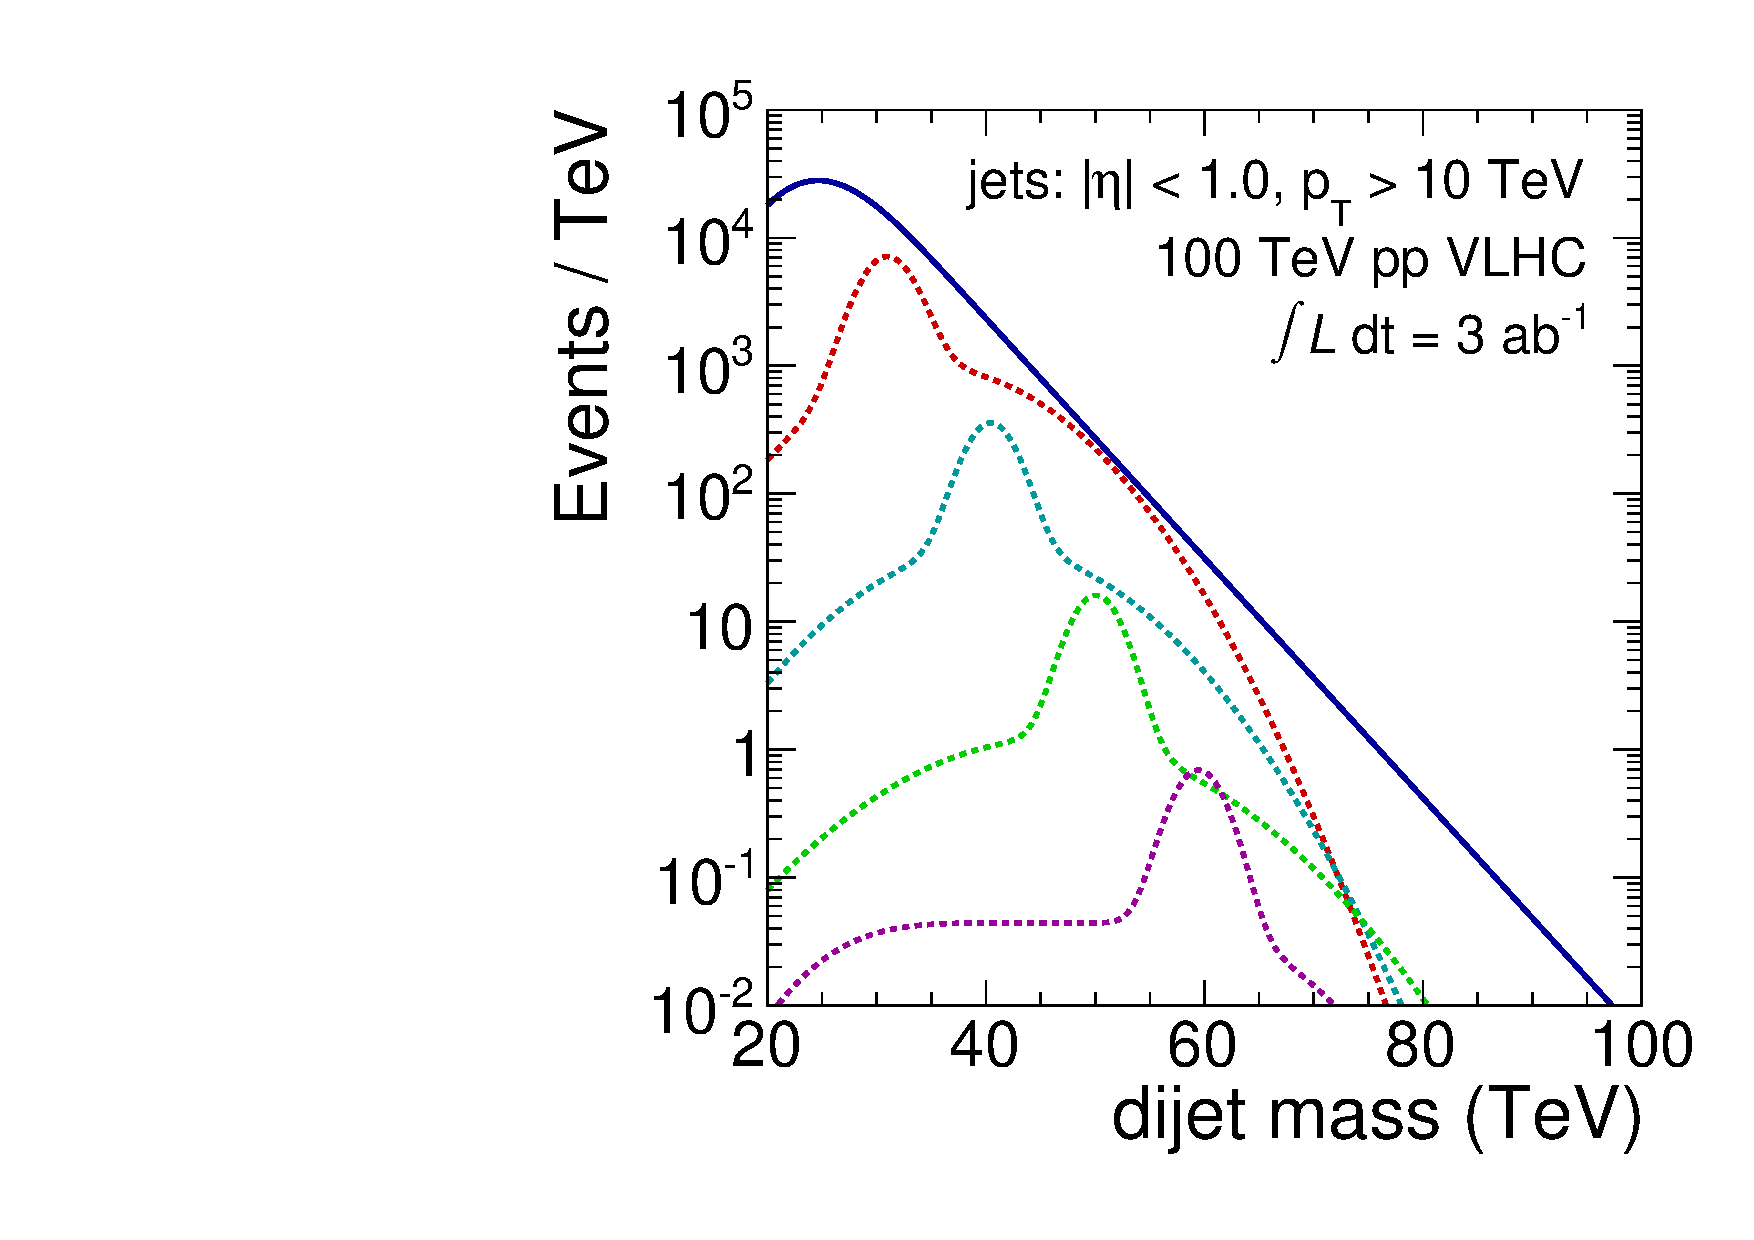
\includegraphics[width=0.475\textwidth]{QstarVLHC/plots/qstar_100TeV}
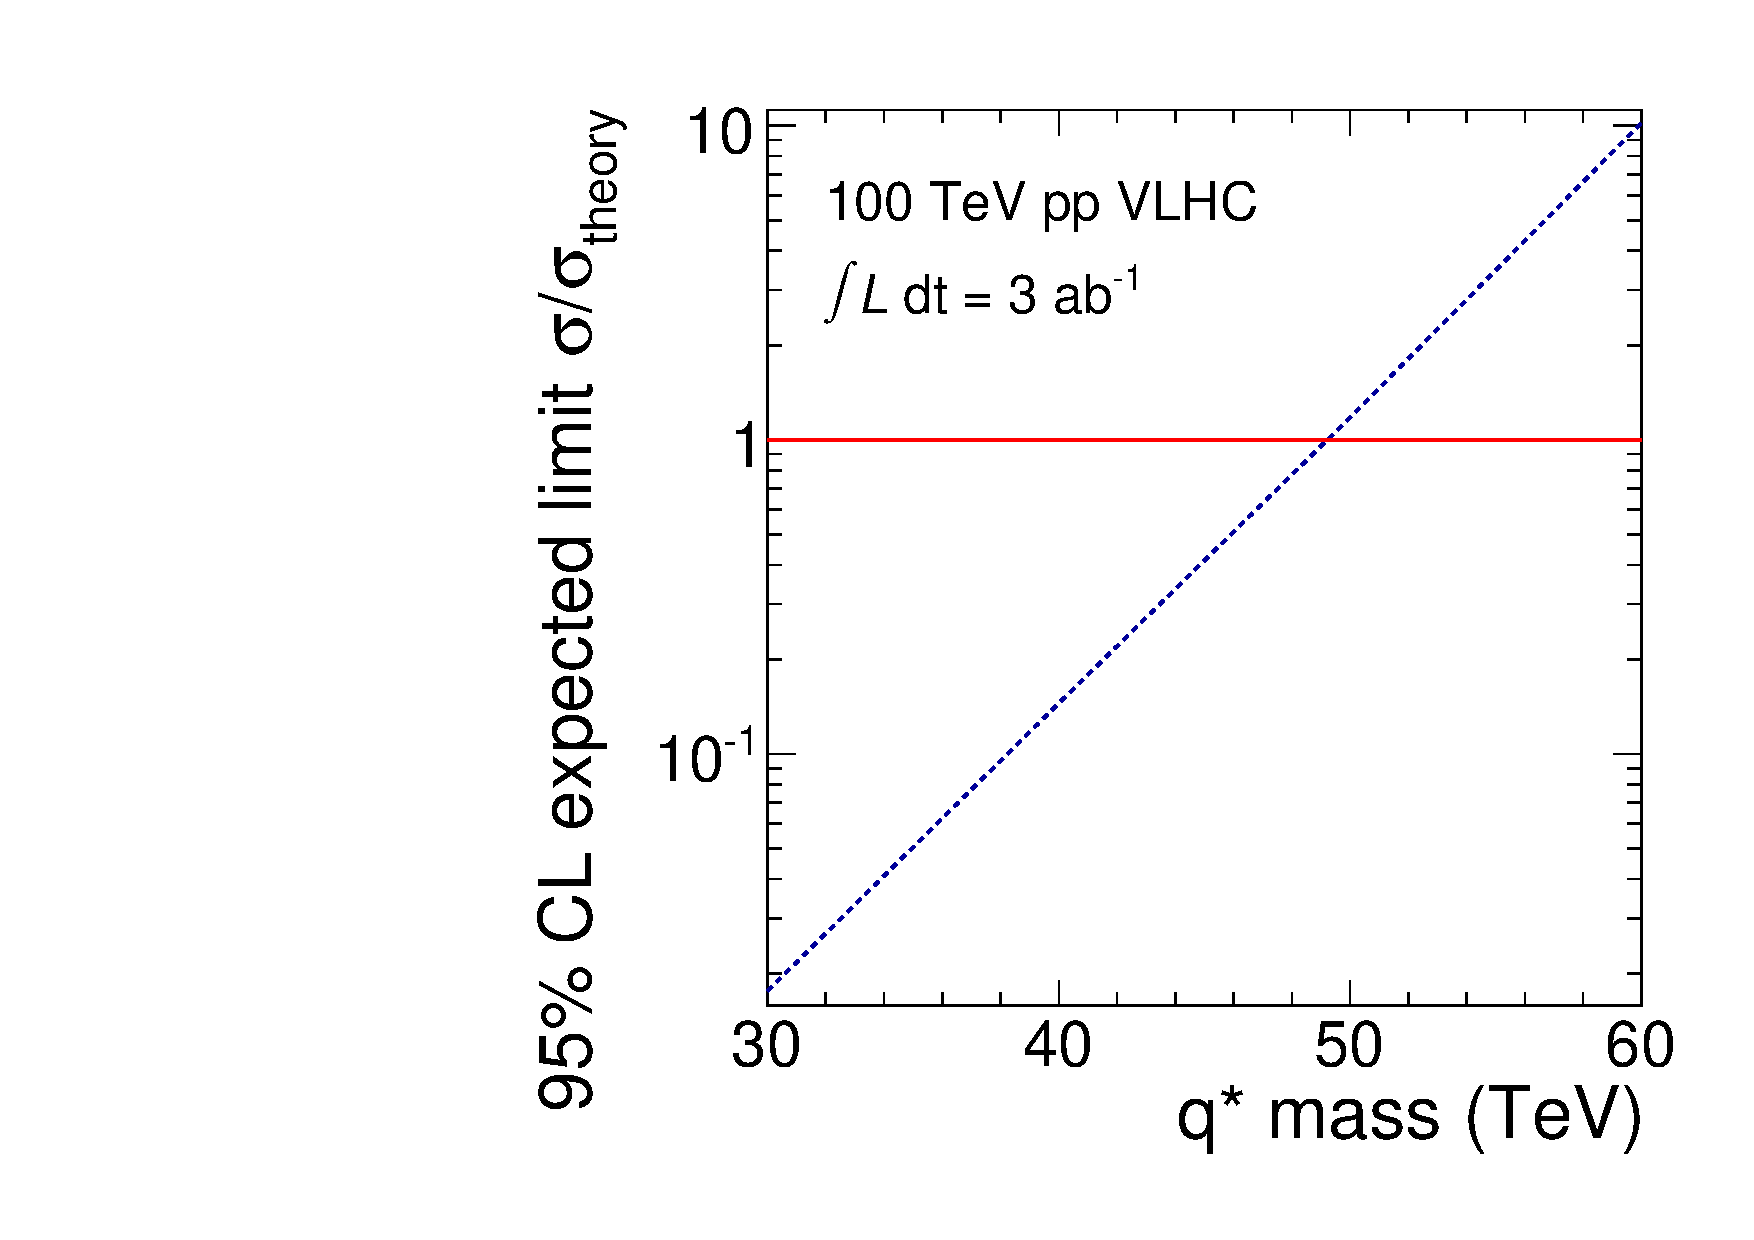
\includegraphics[width=0.475\textwidth]{QstarVLHC/plots/qstar_limits}
\end{center}
\caption{\label{fig:qstar_vlhc}(left) Dijet mass spectrum for
  background dijet production (solid blue line) and $q^*$ models with
  masses from 30\,TeV to 60\,TeV (dashed colored lines). (right) 95\%
  CL upperlimit on the cross-section of $q^*$ resonance as a function
  of its mass normalized by the theoretical prediction for the
  cross-section.}
\end{figure}

\begin{thebibliography}{99}

\bibitem{Baur:1989kv} 
  U.~Baur, M.~Spira and P.~M.~Zerwas,
  %``Excited Quark And Lepton Production At Hadron Colliders,''
  Phys.\ Rev.\ D {\bf 42}, 815 (1990).

\end{thebibliography}


